% Branch and bound tree for maximize knapsack
\tikzset{
  S/.style = {draw, rectangle, rounded corners=0.1cm, minimum size = 8mm,  top color=blue!10, bottom color=blue!10},% top color=white, bottom color=blue!20},
}
     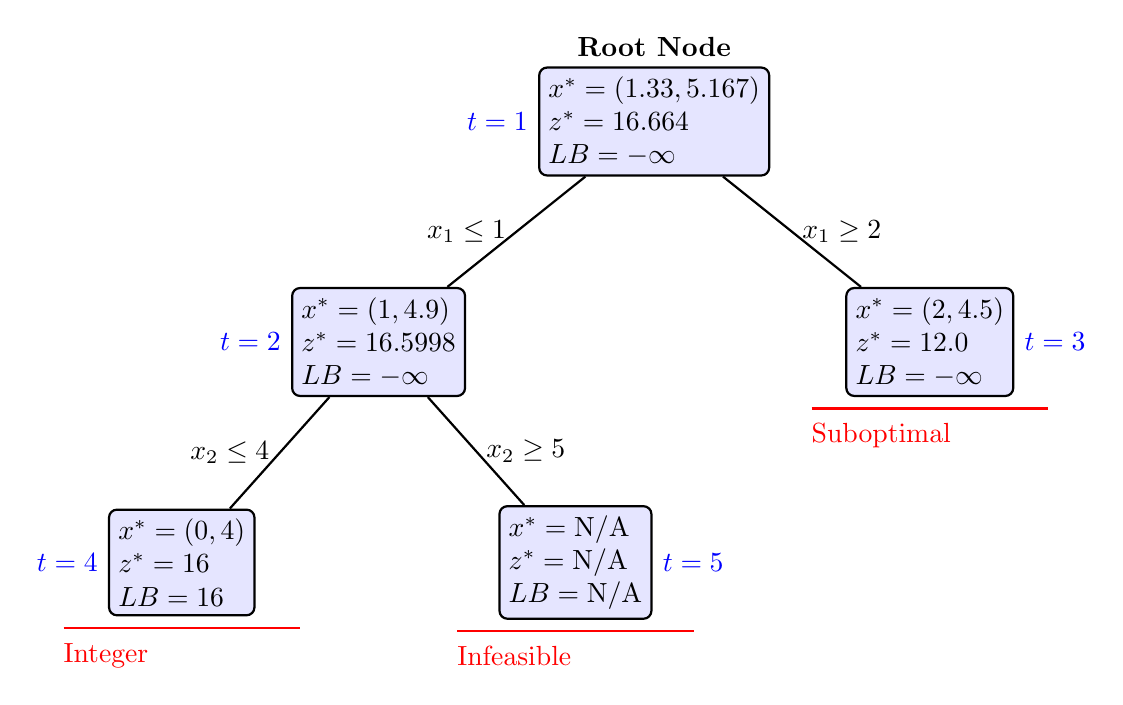
\begin{tikzpicture}[-,thick]
\node[S,sibling distance=5cm, level distance=1.3cm, align=left, label={[blue]left:$t = 1$}, label = {above:\textbf{Root Node}}] 
	{$x^* = (1.33, 5.167) $\\ $z^* = 16.664$\\ $ LB = -\infty$} 
	[sibling distance=7cm, level distance=2.8cm,align=left]
	%
     	child {node[S, label={[blue]left:$t = 2$}] 
     		{$x^* = (1, 4.9) $\\$z^* = 16.5998$\\$ LB = -\infty$}
		[sibling distance=5cm, level distance=2.8cm,align=left]
		child {node[S, label={[blue]left:$t = 4$}, label = {[red]below: \rule{3cm}{0.8pt} \\ \centering Integer}] {$x^* = (0,4)$\\$z^* = 16$\\$ LB = 16$}
		%
     			edge from parent node[left] {$x_2 \leq 4$}}
			%
			child {node[S, label={[blue]right:$t =5$}, label = {[red]below: \rule{3cm}{0.8pt} \\ \centering Infeasible}] {$x^* = \textrm{N/A}$\\$z^* = \textrm{N/A}$\\$ LB = \textrm{N/A}$}[sibling distance=5cm, level distance=2.8cm,align=left]
			%
			edge from parent node[right] {$x_2 \geq 5$}
			}
%
   		edge from parent node[left] {$x_1 \leq 1$}
   }
     child {node[S, label={[blue]right:$t =3$},label = {[red]below: \rule{3cm}{0.8pt} \\ \centering Suboptimal}] 
     		{$x^* = (2, 4.5) $\\$z^* = 12.0$\\$ LB = -\infty$}
		[sibling distance=5cm, level distance=2.8cm,align=left]
		%
   		edge from parent node[right] {$x_1 \geq 2$}
   };

     \end{tikzpicture}
